\section{The Large Hadron Collider}

The Large Hadron Collider (LHC) \cite{Evans:2008zzb,Bruning:2004ej} is a colliding-beam accelerator 
of circulating beams of protons
or lead ions. 
It sits beneath the French-Swiss border outside of Geneva, in the 27-km-circumference tunnel that was originally used
for the Large Electron-Positron collider (LEP). 
 The LHC consists of two beam pipes which house counter-circulating beams.

The protons that collide in the LHC are ionized hydrogen atoms that are bunched in groups
of approximately $1.5\times10^{11}$ protons. To achieve their final energy of 4 TeV per proton,
the proton bunches undergo a series of acceleration steps before being injected into
the main LHC ring, as ilustrated in Fig. \ref{fig:accelerators}.

\begin{figure}[htbp]
\centering
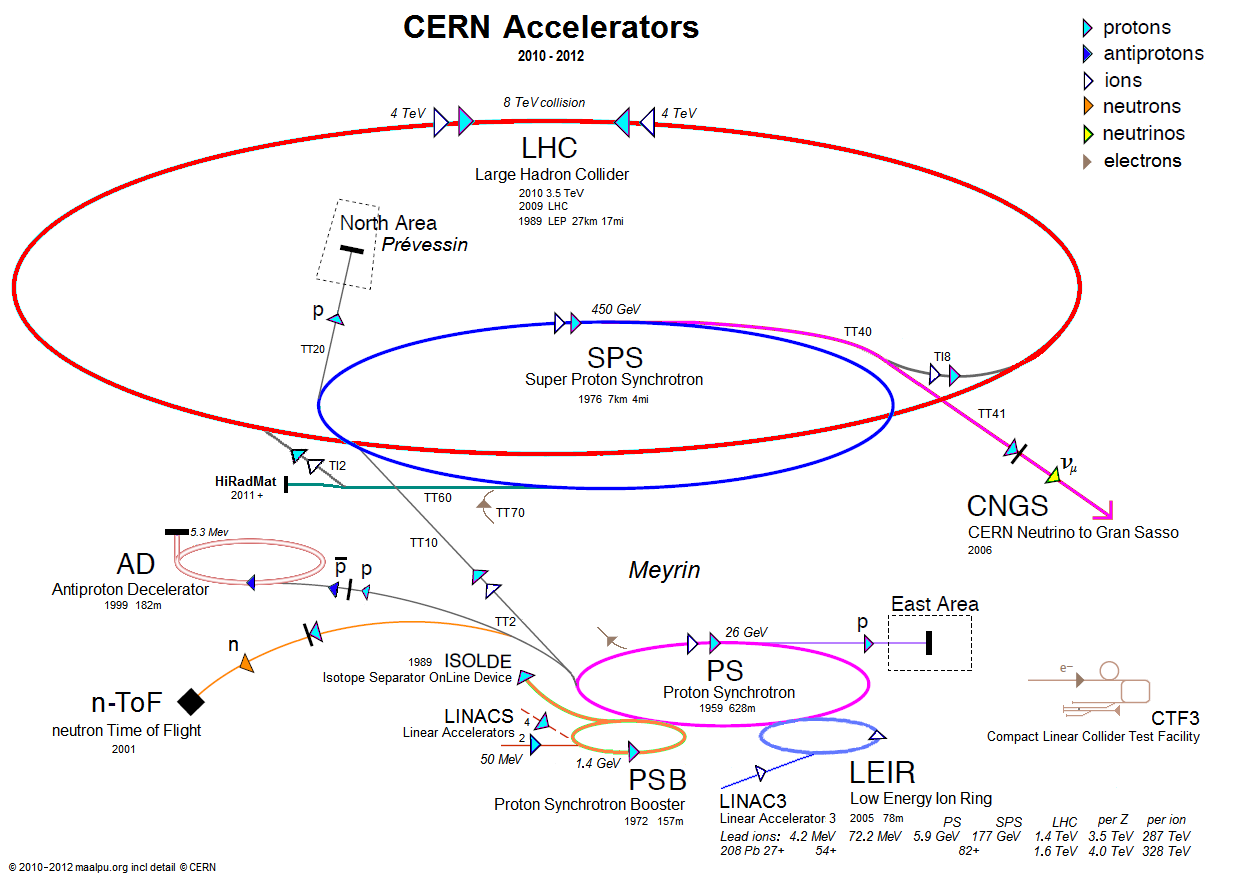
\includegraphics[width=0.9\textwidth]{plots/intro/accelerators.png}
\caption{A schematic diagram of the LHC accelerator complex.\label{fig:accelerators}}
\end{figure}

First, the protons are accelerated in the linear accelerator (LINAC) and injected into 
the Booster where they reach a kinetic energy of 1.4\GeV. The protons are then injected
in the Proton Synchrotron (PS) where the beams are arranged into bunches
with 25~ns or 50~ns spacing, and accelerated to 25\GeV. At the next step
 proton bunches are injected
into the Super Proton Synchrotron (SPS) where they achieve energies of 450\GeV. Finally, the proton
bunches are injected into the LHC. Both LHC beams are fed from the SPS through a series of injections
until a desired number of bunches is reached in both LHC rings. Then, with accelerating 
radio-frequency cavities the beams are brought to the desired operating energies.
The center of mass collision energy for which the LHC was designed, namely 14\TeV,
 is planned to be achieved in 2015.
In 2012 the LHC operated at a reduced energy of 4\TeV per proton, for a total
center of mass energy of $\sqrt{s} = 8 \TeV$.

The beams are steered through the LHC 
using a series of 1232 superconducting dipole magnets with magnetic fields 
of up to 5.5~T for beam energy of 4\TeV. In order to provide superconductivity the 
dipoles are kept at 1.9~K using superfluid helium.
In addition to the dipoles, there are 400 quadrupole magnets used
for focusing the beams.

The LHC beams are
crossed in four sections around the ring to enable collisions of the beams. Each interaction point
houses a large detector, two general purpose ones ATLAS and CMS, and two specialized detectors
ALICE and LHCb. The ALICE and LHCb experiments took advantage of already available caverns from
the LEP experiments, while ATLAS and CMS, located at opposite sides of the LHC ring, as illustrated
in Fig. \ref{fig:lhc}, are located in caverns built specifically for them.

\begin{figure}[htbp]
\centering
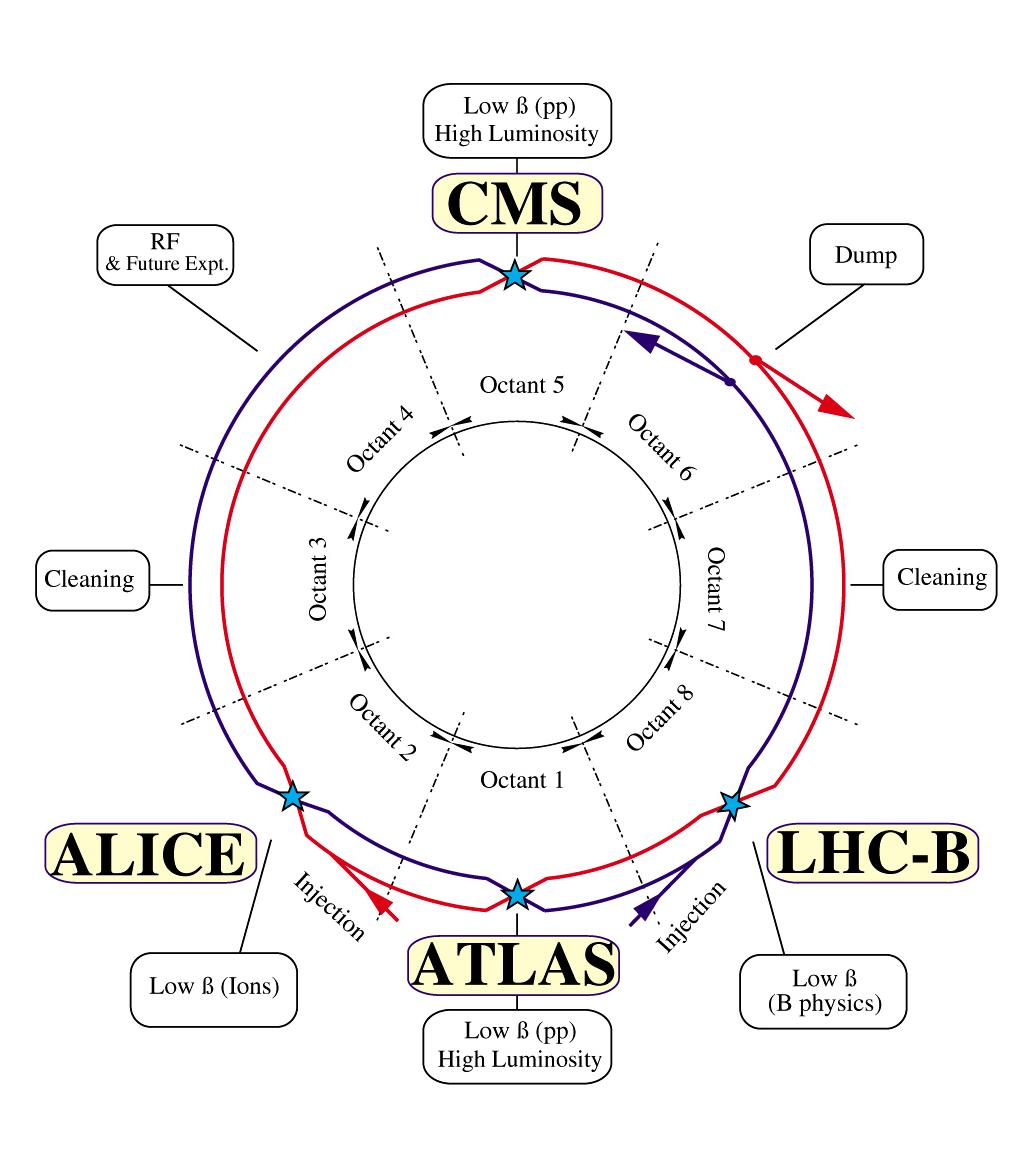
\includegraphics[width=0.6\textwidth]{plots/intro/lhc.jpg}
\caption{The layout of the LHC interaction points.\label{fig:lhc}}
\end{figure}

The instantaneous luminosity of the machine, \ie the rate of scattering events produced divided
by the cross section of the process, is given by \cite{Aaij:2011er}:
\begin{equation}
\mathcal{L}=\frac{f n_b N_p^2}{A_{\mathrm{eff}}}
\end{equation}
where $f$ is the orbit frequency ($\sim$11~kHz), $n_b$ is the number of colliding bunch pairs, 
$N_p$ is the number of protons per bunch, and $A_{\mathrm{eff}}$ is the area in which the bunches
overlap, transverse to the beam directions.


\begin{figure}[htbp]
\centering
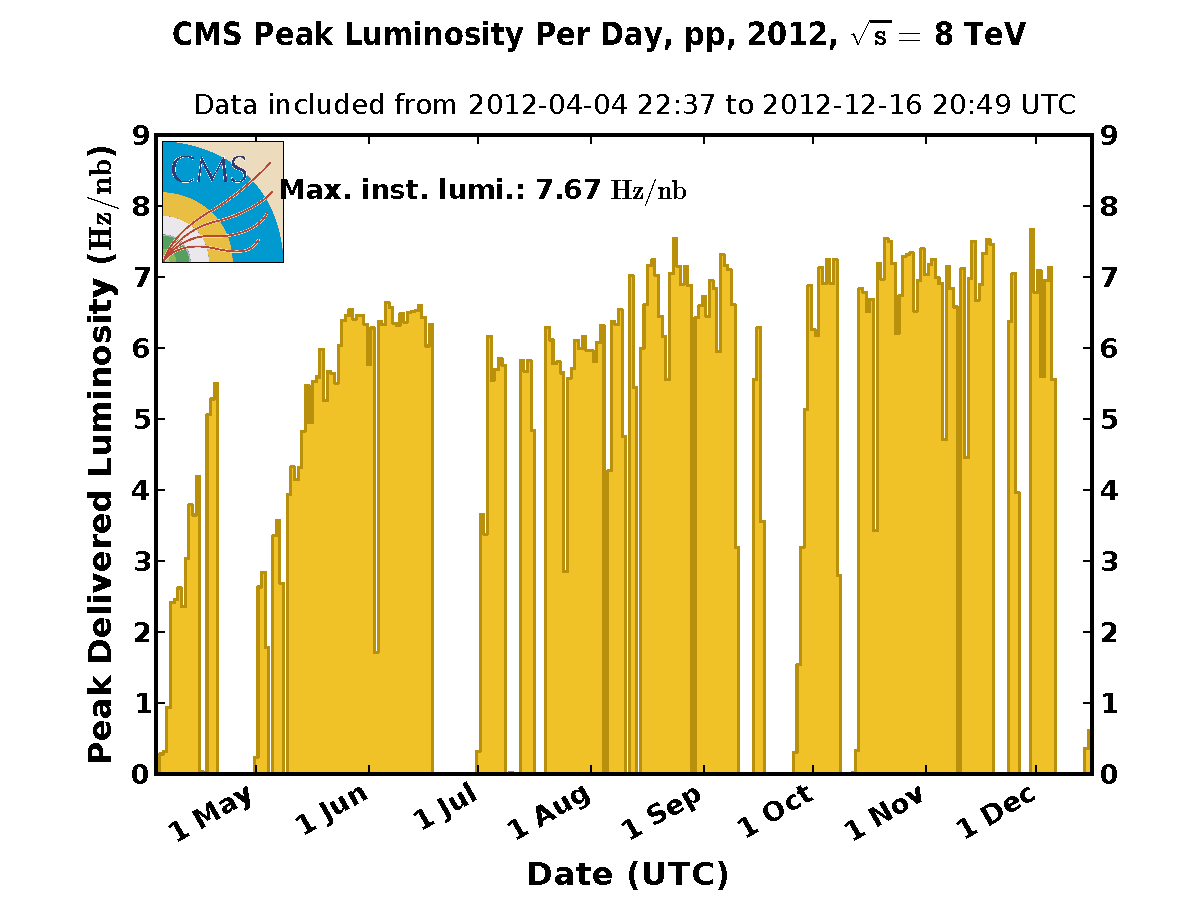
\includegraphics[width=0.49\textwidth]{plots/intro/peak_lumi.pdf}
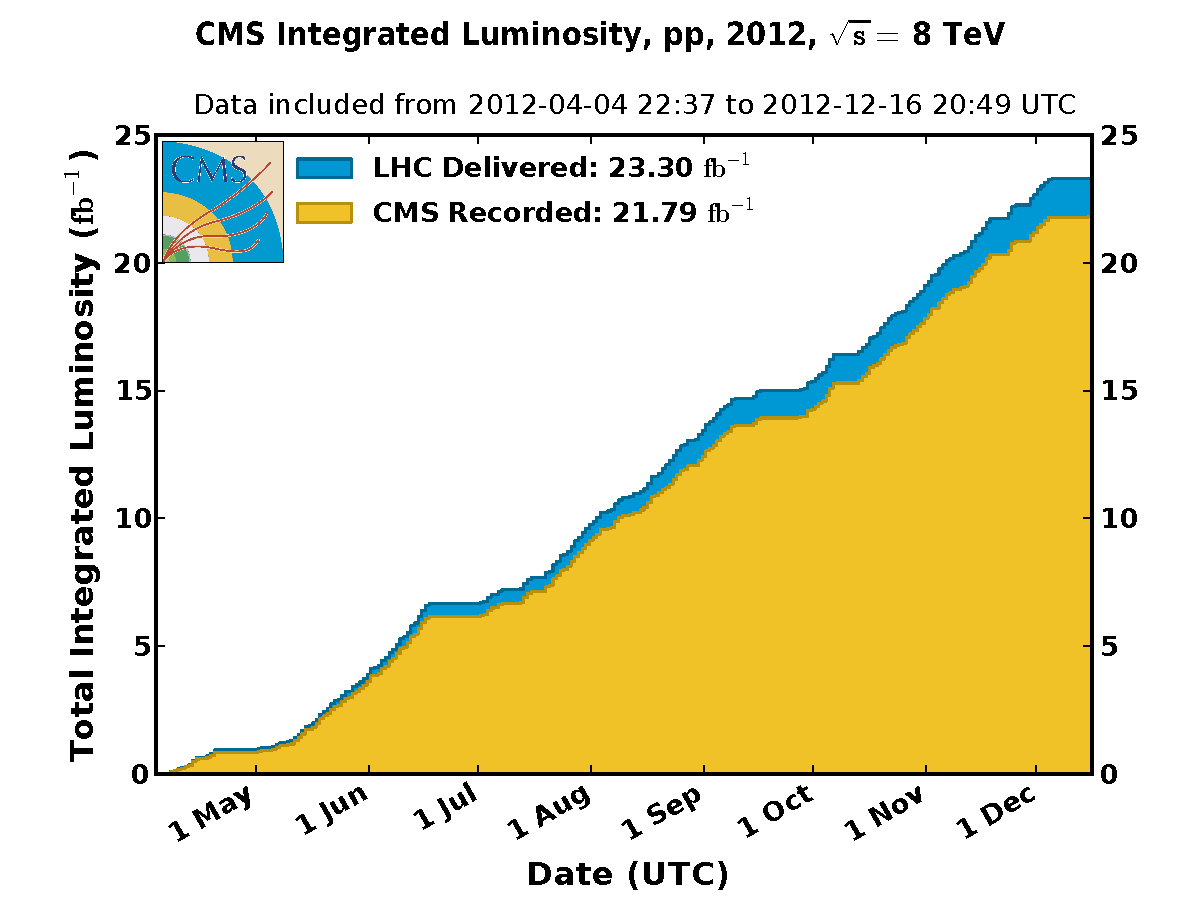
\includegraphics[width=0.49\textwidth]{plots/intro/int_lumi.pdf}
\caption{The daily peak instantaneous luminosity (left) and the integrated luminosity (right)
 delivered to the CMS experiment during the 2012 8\TeV proton-proton run.\label{fig:lumi}}
\end{figure}

The peak instantaneous luminosity per bunch during the 2012 LHC run 
 reaches 7~Hz/$\mu$b, Fig. \ref{fig:lumi}. 
Assuming a hard scattering cross section of $\sim70$~mb, there are $\sim$30 simultaneous interactions 
for each 
crossing of the proton bunches. Simultaneous presence of multiple proton-proton ($pp$) interactions
 poses a significant challenge in the form of difficult event reconstruction and analysis tasks.
 The total integrated luminosity 
delivered to the experiments in the 2012 LHC run of 23.3 \fbinv 
is the highest integrated luminosity for a hadron collider 
to date.
